\documentclass[12pt,answers]{exam}
\usepackage[utf8]{inputenc}
\usepackage{amsfonts,amsthm,amsmath, amssymb, mathtools}
\usepackage[colorlinks=true]{hyperref}
\usepackage[a4paper, margin=0.75in]{geometry}
\usepackage{graphicx}

\title{\vspace{-2em}COL202 Homework 2\vspace{-0.3em}}
\author{Aniruddha Deb, Prabal Singh\vspace{-1em}}
\date{October 2021}
\unframedsolutions

\renewcommand{\solutiontitle}{\vspace{-1em}\noindent\textit{Solution:}\enspace}

\begin{document}
\maketitle
\pagestyle{empty}
\begin{questions}

\question Let $F_1=(V,E_1)$ and $F_2=(V,E_2)$ be any two acyclic graphs (a.k.a.\ forests) on the same vertex set $V$ such that $|E_1|<|E_2|$. Prove that there exists an edge $e\in E_2\setminus E_1$ such that $F=(V,E_1\cup\{e\})$ is also an acyclic graph.
\begin{solution}
Note that the maximum value of $|E_2|$ is $n-1$, in which case $F_2$ will have only 1 connected component. Since $|E_1|<|E_2|$, $F_1$ must have more than 1 connected component. (You need $n-1$ edges to form a connected graph)

Consider a set $S = \{ \{ u,v \} : \{ u,v \} \in E_1 \setminus E_2$ and u and v are vertices in different connected components of $ F_1\}$

We claim that S is non empty.

\begin{proof} Proceed by contradiction. Suppose S is empty. Let $C_i$ be the set of vertices of the $i^{th}$ of the $k$ connected components of $F_1$. If $S$ is empty, this means all the edges in  $E_1 \setminus E_2$ have both end points in a single $C_i$ for any $i$ from $1$ to $k$. This means the sets of all the vertices in the connected components of $F_2$ are subsets of $C_i$'s for $i \in \{1,\ldots,k\}$, since there are no edges that connect 2 connected components of $F_1$. Hence, the maximum number of edges in $F_2$ is $|E_1|$. This is a contradiction since $|E_1|<|E_2|$. Hence S is non-empty.
\end{proof}

Pick any edge from S. If we add this edge to $F_1$ it will join two connected components. From the cut property of trees, we know that if we join two vertices from 2 acyclic connected components which were created by removing an edge from a tree, we get a tree. Hence no cycle is created. Also $F_1$ now has $k-1$ connected components. Therefore, such an edge $e \in E_2 \setminus E_1$ exists.
\end{solution}

\question Prove that every connected graph $G=(V,E)$ has a closed walk which traverses every edge in $E$ exactly twice. Hence, prove that every connected graph $G=(V,E)$ has a closed walk of length $2|V|-2$ which visits every vertex in $V$ at least once.
\begin{solution} Proceed by induction on the number of vertices $|V|$. 

\underline{Base Case:} $|V| = 1$. The claim is true, since there are no edges.

\underline{Induction Hypothesis:} Assume that the claim holds for every connected graph with $k-1$ vertices.

\underline{Induction Step:} Consider a connected graph $G = (V,E)$ with $|V|=k$. Pick an arbitrary vertex $u$ and call it's neighbors $v_1,\ldots,v_m$. If we remove vertex $u$ and its $m$ edges $\{u,v_1 \},\ldots \{u,v_m \}$, we get a graph with $k-1$ vertices. From the induction hypothesis, the new graph contains a closed walk that traverses each edge twice. $v_1,\ldots,v_m$ will all appear at least once in the closed walk sequence. This is because there must be some edge connecting them. Replace the last occurrence of each $v_i$ with $v_i u v_i$. This way all the 'new' (edges which were absent in the $k-1$ vertex graph) edges in the graph $G$ will now be traversed twice. Hence, the claim is true for a graph with $k$ vertices. \hfill $\square$

For the second part, since the graph $G$ is connected there exists a spanning tree for the graph (proved in lecture). The number of edges in this spanning tree would be $|V|-1$, and by the above proof, there would be a closed walk which traverses each edge twice, and since the graph has edges connecting all the vertices, each vertex is visited at least once. The length of this closed walk would be $2(|V|-1) = 2|V|-2$. 
\end{solution}


\question A graph is said to be \textit{regular} if the degrees of all its vertices are the same, A matching $M$ in a graph is said to be a \textit{perfect matching} if for every vertex $v$, $M$ contains an edge incident on $v$ (that is, all vertices are matched by $M$). Prove that the edge set of every bipartite regular graph can be partitioned into perfect matchings. (Convince yourself that the claim is not true if the graph is (i) regular but not bipartite, even if it has an even number of vertices (ii) bipartite but not regular, even if the gtaph is connected, both sides of its bipartition contain an equal number of vertices, and the degree of every vertex is at least $d$, where $d$ is as large a constant as you want.)
\begin{solution} We first prove the following lemma

\underline{Lemma:} Every regular nonempty bipartite graph has an even number of vertices

\begin{proof}
Proceed by contradiction: suppose $G = (V,E)$ is a bipartite graph with an odd number of vertices $n$. Partition $V$ into two sets $S_1$ and $S_2$, and WLOG assume $|S_1| > |S_2|$ (Equality is impossible because $n$ is odd). By pigeonhole principle, there would be atleast one edge between two vertices in $S_1$, giving us a contradiction. Hence, $n$ has to be even.
\end{proof}

Now, proceed by strong induction on the number of vertices $2n$ of a regular nonempty bipartite graph

\underline{Base case:} $n = 1$. The only graph possible is two vertices with one edge between them, which has only one possible perfect matching.

\underline{Induction Hypothesis:} Assume that every regular nonempty bipartite graph with less than or equal to $2(n-1)$ edges has a perfect matching.

\underline{Induction Step:} Consider the regular nonempty bipartite graph $G = (V,E)$ with $2n$ vertices, partitioned into $S_1$ and $S_2$ such that $|S_1| = |S_2| = n$. Take any two vertices $u \in S_1$, $v \in S_2$ such that $\{u,v\} \in E$. Make a matching between these two vertices. Assuming that the degree of every vertex is $k$, we now have three regular bipartite subgraphs of $G$:
\begin{enumerate}
    \item $G_1$, with $2(n-k)$ vertices, each of degree $k$. These are the vertices that were not connected to $u$ or $v$
    \item $G_2$, with $2(k-1)$ vertices, each of degree $k-1$. These are the vertices that were connected to either $u$ or $v$
    \item $G_3$, with $2$ vertices $u,v$ and one edge $\{u,v\}$
\end{enumerate}

By our strong induction hypothesis, all these subgraphs have perfect matchings $M_1, M_2, M_3$, and hence the perfect matching of $G$ is simply $M_1 \cup M_2 \cup M_3$. \hfill $\square$
\end{solution}

\question Find an expression for the number of perfect matchings in a complete graph on $n$ vertices, and prove your answer. Your expression must involve only a constant number of applications of only the following mathematical operators: addition, subtraction, multiplication, division, exponentiation, and factorial.
\begin{solution}
For a complete graph with an odd number of vertices, there does not exist a perfect matching, because there will always be one vertex that is not matched. Hence, the number of perfect matchings if $n = 2k-1$ is $\boxed{0}$

If $n = 2k$, then the number of perfect matchings is the number of ways to divide $2k$ vertices into $k$ sets of $2$ vertices each (this is because the graph is complete, and hence there exists an edge between every pair of vertices). The number of ways to do this is to choose two out of the first $2k$, then two out of the remaining $2k-2$, then two out of the remaining $2k - 4$ and so on. Since this gives us the matching in a specific order, this is equal to the $k!$ ways of permuting the matchings. The number of perfect matchings is thus 
\begin{align*}
    k! N &= \binom{2k}{2}\binom{2k-2}{2}\cdots\binom{2}{2} \\
      &= \frac{(2k)!}{2!(2k-2)!}\ \frac{(2k-2)!}{2!(2k-4)!}\ \cdots \frac{2!}{2!0!} \\
      &= \frac{(2k)!}{(2!)^k} \\
    \Aboxed{N &= \frac{(2k)!}{(k!)2^k}}
\end{align*}
\end{solution}

\question Consider a Delhi Metro train consisting of $n$ seats numbered $1,\ldots,n$ carrying $m$ (distinct) passengers. The government rules for physical distancing prevent passengers from standing in the compartment during their journey. Moreover, they must leave a gap of at least two seats between themselves: if a seat $k$ is occupied, seats $k-2$, $k-1$, $k+1$, $k+2$ must remain vacant. Find an expression for the number of ways in which the passengers can occupy seats while following the physical distancing norms, and prove your answer. Again, your expression must involve only a constant number of applications of only the following mathematical operators: addition, subtraction, multiplication, division, exponentiation, and factorial.
\begin{solution}
Rather than distributing $m$ passengers in $n$ seats, we assign one seat to each of the $m$ passengers and then distribute the remaining $n-m$ seats in such a way that the passengers are socially distanced. The arrangement of seats is then as follows:

\begin{center}
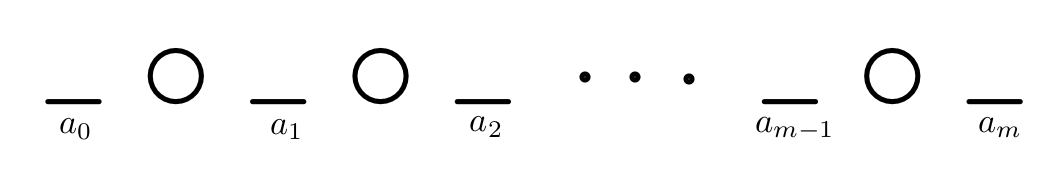
\includegraphics[width=4in]{seats.png}
\end{center}

Here, $a_0, a_m \ge 0$ and $a_1, a_2, \ldots a_{m-1} \ge 2$. Hence, if we distribute 2 seats in each of $a_1, a_2, \ldots a_{m-1}$, we are left with $n-m-2(m-1) = n-3m+2$ identical seats to distribute in $m+1$ identical boxes with empty boxes allowed. The number of ways of doing this is $^{n-2m+2}C_m$ (provided $n-3m+2 \ge 0$, otherwise it is $0$). Since the passengers are distinct, once their positions are fixed, we can shuffle them in $m!$ ways. Hence, the total number of ways of distributing passengers is 
$$N = \begin{cases}
\frac{(n-2m+2)!}{(n-3m+2)!} & n-3m+2 \ge 0 \\
0 & n-3m+2 < 0
\end{cases}$$
\end{solution}

\end{questions}
\end{document}
